\begin{tikzpicture}
    \begin{scope}[shift={(-2,0)}]
        % \draw [step=0.1,very thin, yellow] (-2,-2) grid (2,2);
        % \draw [step=0.5,very thin, red] (-2,-2) grid (2,2);
        % \draw [very thin, green] (-2,-2) grid (2,2);
        \begin{scope}
            \clip (-1.8,-1.5) rectangle  +(3.6,3);
            \node[inner sep=0pt] at (4.7,1.5)
                {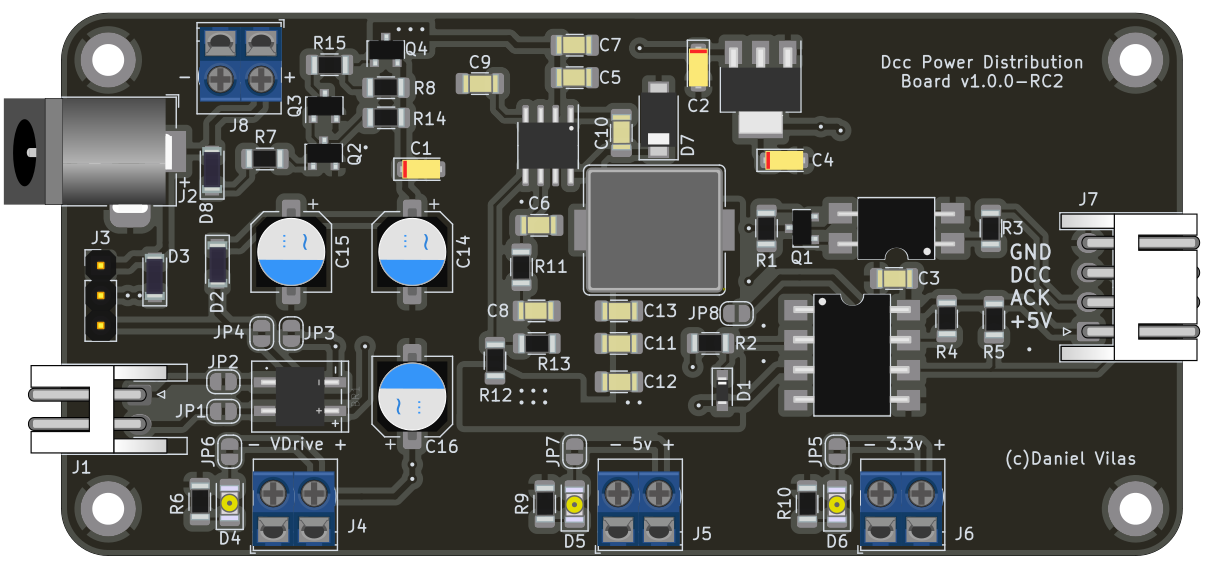
\includegraphics[scale=1.3]{images/front.png}};
        \end{scope}
        \draw[yellow,line width=2pt,rounded corners=4pt] 
            (-0.2,-0.1) rectangle +(1,0.95);
        
            \node[below] at (0,-2) {(a) JP1 y JP2};

        %\draw[white] (-2,0)--(2,0);
    \end{scope}
    \begin{scope}[shift={(3,0)}]
        % \draw [step=0.1,very thin, yellow] (-2,-2) grid (2,2);
        % \draw [step=0.5,very thin, red] (-2,-2) grid (2,2);
        % \draw [very thin, green] (-2,-2) grid (2,2);
        \begin{scope}
            \clip (-1.8,-1.5) rectangle  +(3.6,3);
            \node[inner sep=0pt] at (4.7,1.5)
                {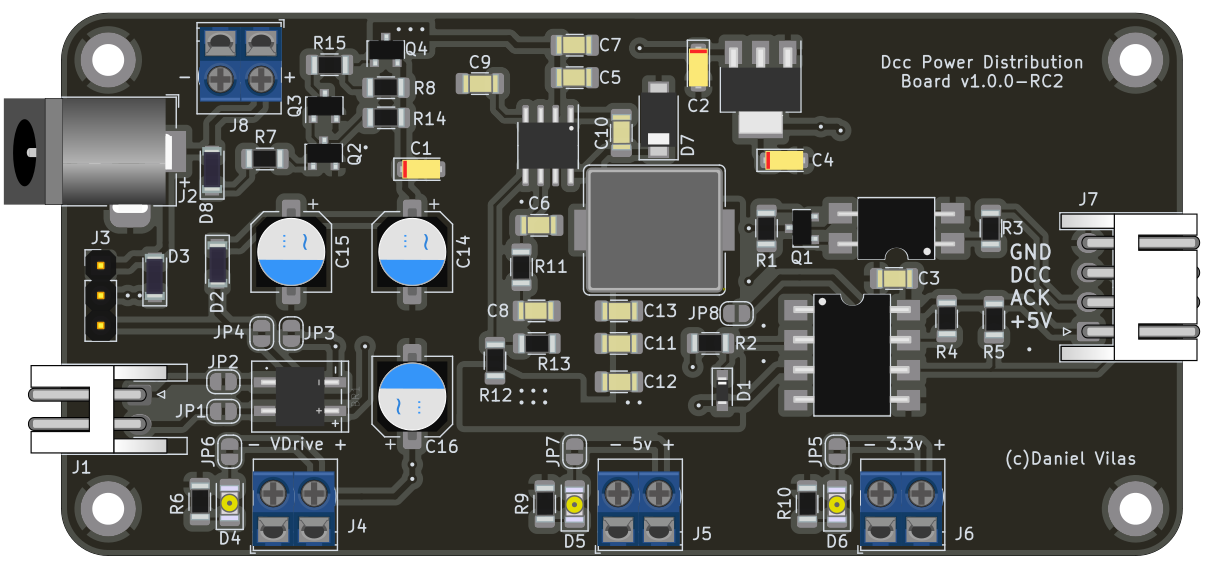
\includegraphics[scale=1.3]{images/front.png}};
        \end{scope}
        \draw[yellow,line width=2pt,rounded corners=4pt] 
            (0.25,0.7) rectangle +(1.5,0.55);
        
            \node[below] at (0,-2) {(b) JP3 y JP4};

        %\draw[white] (-2,0)--(2,0);
    \end{scope}
\end{tikzpicture}